\documentclass[output=paper]{langsci/langscibook}
\ChapterDOI{10.5281/zenodo.4680308}

\author{Anders Holmberg\affiliation{University of Newcastle}}
\title{Case and agreement in possessive noun phrases in mainly English, Swedish,
and Finnish}
\rohead{\thechapter\hspace{0.5em}Case and agreement in possessive noun phrases}

\abstract{The paper is based on a set of observations about the prenominal
    possessive construction in \ili{English}, \ili{Swedish}, \ili{Finnish}, and \ili{Hungarian}. These
    include the fact that \isi{coordination} of possessive pronouns is degraded in
    \ili{English} (??\emph{your and my home}), but not in the other languages and
    that the adnominal pronoun construction (APC) \emph{we children} cannot
    have a genitive\is{genitive case} pronoun in \ili{English} or \ili{Swedish}
    (*\emph{our children home}) but can do in \ili{Finnish}. On the other hand
    \ili{Finnish} and \ili{Hungarian} do not show possessive agreement when the
    possessor is an APC\@. These observations can be explained if the
    possessive construction has the structure [Poss [\textsubscript{NP} DP N]],
    where Poss hosts a set of unvalued \isi{φ-features} valued by the possessor DP\@.
    In \ili{English} and \ili{Swedish}, Poss is spelled out as a genitive\is{genitive
    case} pronoun (\emph{my}, \emph{her}, \emph{our}, etc.). In \ili{Finnish}
    and \ili{Hungarian} it is spelled out as a possessive agreement suffix.  In
    all the languages this is the case only when the possessor DP is a bare
pronoun: Poss does not agree with a lexical DP\@.  This is couched in a version
of the theory of agreement and incorporation in
\textcite{Roberts2010,Roberts2010b}.}


\begin{document}\glsresetall
\maketitle
\multicolsep=.25\baselineskip

%\textbf{Keywords:} agreement, Agree, possessive, pronoun, incorporation

\section{Introduction}\label{sec:16.1}

This paper is based on mainly two observations about possessive noun phrases in
English, \ili{Swedish}, and \ili{Finnish}. The first one is that \isi{coordination} of possessive
pronouns is degraded in \ili{English}, for most combinations, but perfectly well
formed in \ili{Swedish} and \ili{Finnish}.\newpage

\ea\label{ex:16.1}
	\ea English\\
    ?? my and your friends
	\ex \ili{Swedish}\\
		\gll mina och dina vänner\\
        my    and your friends\\
    \ex \ili{Finnish}\\
		\gll minun ja  sinun ystävät\\
        my and your friends\\
	\z
\z

The second observation concerns the \glsunset{APC}\glsdesc{APC}
(\gls{APC}\is{adnominal pronoun construction}:\is{APC|see{adnominal pronoun construction}}
\emph{you children, we linguists}). Ever since \textcite{Postal1969} it has been widely
accepted that the adnominal pronoun is a determiner taking the lexical noun as
its complement, and ever since \citet{Abney1987} it has been widely accepted
that the determiner is the head of the argument noun phrase.  As the head, the
pronoun in the \gls{APC}\is{adnominal pronoun construction} will reflect the case assigned to the DP; it is
\emph{we children} if the DP is subject, \emph{us children} if the DP is
object.\footnote{ This is the Standard \ili{English} rule. There is variation in
English regarding nominative\is{nominative case} vs.\ accusative in various
contexts. See below \cref{fn:16.2} and discussion of \eqref{ex:16.8}.} However when the
\gls{APC}\is{adnominal pronoun construction} is a possessor, the pronoun does not have genitive\is{genitive case} (possessive) case,
in \ili{English}. The \gls{APC}\is{adnominal pronoun construction} rather behaves as a lexical DP possessor, constructed
(somewhat marginally) with the possessive clitic \emph{-s}.

\ea\label{ex:16.2}
    \ea[*]{your children opinions}
    \ex[?]{you children’s opinions}
	\z
\z

In \ili{Swedish}, too, the possessive pronoun cannot have genitive\is{genitive case} case.

\ea\label{ex:16.3}\ili{Swedish}\\
    \gll   \llap{*}era                barn       åsikter\\
            you.\Pl{}.\Poss{} children opinions \\
\z

But in \ili{Finnish} the \gls{APC}\is{adnominal pronoun construction} can occur as a possessor with genitive\is{genitive case} case.

\ea\label{ex:16.4}\ili{Finnish}\\
    \gll teidän       lapsien            mielipiteet \\
        you.\Gen{} children.\Gen{} opinions\\
	\glt    `you children’s opinions'
\z

With some qualification, this is also possible in \ili{Hungarian}. Another relevant
observation is that the possessive construction in \eqref{ex:16.4} does not admit possessor
agreement on the noun, while this is optional or obligatory, depending on the
variety of \ili{Finnish}, with a bare possessive pronoun.

\ea\label{ex:16.5}\ili{Finnish}
	\ea
		\gll teidän       mielipitee-nne \\
			you.\Gen{} opinions-\Spl{}\\
		\glt    `your.\Pl{} opinions'
	\ex
		\gll teidän       lapsien             mielipitee (*-nne)\\
            you.\Gen{} children.\Gen{} opinions \hphantom{(*}-\Spl{}\\
		\glt    `you children’s opinions'
	\z
\z

\begin{sloppypar}
These observations will be made sense of with the help of the theory of
agreement and incorporation articulated in \textcite{Roberts2010,Roberts2010b}.
The possessive pronouns in \ili{English} and \ili{Swedish} are possessive determiner
(Poss) heads derived by Agree between Poss and an NP-internal possessor
argument in a structure [\textsubscript{Poss/DP} Poss NP]; this is how they are
Case-licensed. If the possessor is lexical, Poss does not agree with it, but is
spelled out as the invariant clitic –s. The possessor in \ili{Finnish} is
assigned genitive\is{genitive case} case in the NP. If the possessor is a
pronoun, it undergoes Agree with Poss in the structure [\textsubscript{Poss/DP}
Poss NP], spelled out as an agreement suffix on the possessee noun. If the
possessor is lexical, Poss does not agree with it. The \gls{APC}\is{adnominal
pronoun construction}, in spite of being headed by a pronoun, does not trigger
agreement.  In this way the reason why (\ref{ex:16.2}a) and
\eqref{ex:16.3} are ill-formed is the same reason why the possessive
agreement suffix is ill formed in \ili{Finnish} (\ref{ex:16.5}b): they
feature illicit agreement. The reason why (\ref{ex:16.5}b) is well-formed
in \ili{Finnish} without the possessive agreement suffix, unlike
(\ref{ex:16.2}a) and \eqref{ex:16.3}, is that the possessor DP can get
genitive\is{genitive case} case independently. The situation in \ili{Hungarian}
will be touched upon briefly; it is similar, though not identical with the
situation in Finnish.
\end{sloppypar}

\section{The adnominal pronoun construction as possessor}\label{sec:16.2}

The following terminology will be used: a nominal construction with a possessor
and a possessee will be called \emph{possessive construction} or just
\emph{possessive}. The argument with the possessor role will be called
\emph{possessor} or \emph{possessor DP} (ignoring the issue whether nominal
arguments are necessarily DPs in all languages, including \ili{Finnish}, a language
without articles). If it is a pronoun it will be called \emph{possessor
pronoun}.

Ever since \citet{Postal1969} the adnominal pronoun construction (\gls{APC}\is{adnominal pronoun construction}),
exemplified in \eqref{ex:16.6}, has played a crucial role in the theory of
noun phrase structure.

\ea\label{ex:16.6}
	\ea We children should be taken more seriously.
	\ex They look down on us children.
	\z
\z

\citet{Postal1969} used the \gls{APC}\is{adnominal pronoun construction} to
argue that pronouns are determiners taking a lexical NP as complement, where
the lexical NP may be pronounced/spelled out or not. In \citet{Abney1987} this
became part of the argumentation for the DP-hypothesis. The structure of the
\gls{APC}\is{adnominal pronoun construction} would be (\ref{ex:16.7}a),
under this hypothesis (here simplified; see \citealt{Hoehn2017} for a more
detailed analysis), while the structure of a DP with a lexical possessor DP
would be (\ref{ex:16.7}b).

\ea\label{ex:16.7}
    \begin{multicols}{2}\raggedcolumns\ea
    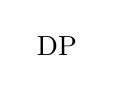
\begin{tikzpicture}[baseline=(root.base)]

        \Tree   [.\node(root){DP};
                    [.D you ]
                    [.N children ]
                ]

    \end{tikzpicture}\columnbreak
    \ex
    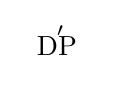
\begin{tikzpicture}[baseline=(root.base)]

        \Tree 	[.\node(root){DP};
                    [.DP \edge [roof]; {the children} ]
                    [.D$'$
                        [.D -s ]
                        [.N friends ]
                    ]
                ]

    \end{tikzpicture}
    \z\end{multicols}
\z

As can be seen in (\ref{ex:16.6}a,b), the pronoun in the
\gls{APC}\is{adnominal pronoun construction} overtly shows the case assigned to
the DP; nominative\is{nominative case} in (\ref{ex:16.6}a), accusative in
(\ref{ex:16.6}b).\footnote{The following is an expression in a Facebook
    message written by a native \ili{English} speaker:  (This was) “a good plug
    for we skipraiders”.  This would be a case where the \isi{accusative case}
    assigned by the preposition does not trickle down to the  head of the
\gls{APC}\is{adnominal pronoun construction}.\label{fn:16.2}} In \ili{English}
the nomina\-tive--accusative distinction is visible only on pronouns.
\ili{English} also has a genitive\is{genitive case} or possessive case visible
on pronouns, as in \emph{my book, our friends}, etc. It is visible only on
pronouns if we take the clitic \emph{–s} in (\ref{ex:16.7}b) to be a
possessive marker of sorts but not a spell-out of genitive case. The possessor
pronoun cannot, however, be constructed as the head of an APC.

\ea\label{ex:16.8}
    \ea[*]{Our children opinions should be taken seriously.}
    \ex[?]{We/us children’s opinions should be taken seriously.}
    \ex[]{We/us children, our opinions should be taken seriously.}
	\z
\z

(\ref{ex:16.8}a) is virtually unparsable. (\ref{ex:16.8}b) may be
somewhat marginal but is very clearly preferable to (\ref{ex:16.8}a),
either with nominative\is{nominative case} or default pronominal accusative on
the pronoun; there appears to be some variation among speakers which option
they prefer. Another clearly well-formed alternative is (\ref{ex:16.8}c),
with a left-dislocated \gls{APC}\is{adnominal pronoun construction} combined
with a possessor pronoun.

The same holds true of \ili{Swedish}. (\ref{ex:16.9}a,b) shows that \ili{Swedish}
has the \gls{APC}\is{adnominal pronoun construction}, with
case visible on the pronoun.\largerpage[-2]

\ea\label{ex:16.9}\ili{Swedish}
	\ea
		\gll Vi  barn  borde  tas  mera på allvar.\\
			we children should take.\Pass{} more on serious\\
		\glt    `We children should be taken more seriously.'
	\ex
		\gll Dom ser  ner  på oss barn.\\
			they  look down on us children\\
		\glt    `They look down on us children.'
	\z
\z

(\ref{ex:16.10}a,b) show that the possessor pronoun cannot be constructed as an
APC.\footnote{(\ref{ex:16.10}b) seems even more marginal than (\ref{ex:16.8}b). There is no obvious
explanation for this, in terms of the theory expounded here. It is also not
confirmed by a proper comparative investigation, so I leave it aside here.}

\ea Swedish\label{ex:16.10}
    \judgewidth{??}
    \ea[*]{
		\gll Våra barn  åsikter  tas   inte på allvar.\\
            our  children opinions take.\Pass{} not on serious\\}
    \ex[??]{
		\gll Vi  barns  åsikter  tas  inte på allvar.\\
			we children’s opinions take.\Pass{} not on serious\\
        \glt    `We children’s opinions are not taken seriously.'}
    \ex[]{
		\gll Vi barn,  våra åsikter  tas  inte på allvar.\\
			we children our opinions take.\Pass{} not  on serious\\
        \glt    `We children, our opinions are not taken seriously.'}
	\z
\z

Standard \ili{Swedish} has the possessive construction in (\ref{ex:16.7}b) with
lexical possessors, essentially just like \ili{English} (see
\citealt{Delsing1998,Julien2005}; virtually the only difference is that the possessive clitic
\emph{–s} is not spelled with an apostrophe in Swedish).\footnote{There is much
dialectal variation in \ili{Swedish}, and Mainland Scandinavian generally, regarding
the possessive construction
\parencite{HolmbergSandstrom1996,Delsing1998,Julien2005}.}
(\ref{ex:16.10}b) would be an instance of that construction. It may be
highly marginal, but is still preferable to (\ref{ex:16.10}a), which is
word salad. (\ref{ex:16.10}c), with a left-dislocated
\gls{APC}\is{adnominal pronoun construction}, is a perfectly well-formed
alternative.\footnote{The \gls{APC}\is{adnominal pronoun construction} does
    not form a constituent together with the possessive pronoun in this case;
    (i) is ill formed.

\begin{exe}
    \exi{(i)}\ili{Swedish}\\
	\gll \llap{*}Dom skrattar åt vi/oss barn våra åsikter.\\
         they laugh at we/us children our opinions\\
\end{exe}}

This is not a universally the case, though. \ili{Finnish} has the \gls{APC}\is{adnominal pronoun construction}, as shown in
\eqref{ex:16.11}.

\ea
    \label{ex:16.11}\ili{Finnish}
	\ea
		\gll Me lapset                      voimme  tulla mukaan. \\
			we.\Nom{} children.\Nom{} can.\Fpl{} come along\\
		\glt    `We children can come along.'
	\ex
		\gll Ne  eivät      ota  meitä    lapsia         vakavasti.\\
			they.\Nom{} not.\Tpl{}  take we.\Part{} children.\Part{} seriously\\
		\glt    `They don’t take us children seriously.'
	\z
\z

The \ili{Finnish} \gls{APC}\is{adnominal pronoun construction}, like any other noun
phrase, has morphological case\is{case!morphological case} on the head noun and on specifiers and
modifiers, in this case on the pronominal determiner. In (\ref{ex:16.11}a)
the case is nominative\is{nominative case}, the case of the subject of finite
clauses. The case on the \gls{APC}\is{adnominal pronoun construction} in
(\ref{ex:16.11}b) is partitive, one of the object cases in \ili{Finnish}. The
possessor case in \ili{Finnish} is genitive.  In possessives with a pronominal
possessor, Standard \ili{Finnish} has possessor agreement in the noun phrase,
realized as a suffix on the noun; see (\ref{ex:16.12}a,b).  The pronoun has
genitive\is{genitive case} case and can be null except in the third person (see
\citealt{BratticoHuhmarniemi2015}). With a lexical possessor, as in
(\ref{ex:16.12}c), there is no agreement (the third person suffix is
neutral for number).

\ea Finnish\\\label{ex:16.12}
	\ea
		\gll (Meidän) mielipiteitä-\textbf{mme} ei   oteta   vakavasti.\\
        \hphantom{(}we.\Gen{} opinions.\Part{}-\Fpl{} not take.\Pass{} seriously\\
		\glt    `Our opinions are not taken seriously.'
	\ex
		\gll Heidän      mielipiteitä-\textbf{nsä} ei oteta  vakavasti.\\
			their.\Gen{} opinions.\Part{}-\Third{} not take.\Pass{} seriously\\
		\glt    `Their opinions are not taken seriously.'
	\ex
		\gll Lapsien mielipiteitä(*-\textbf{nsä})  ei  oteta           vakavasti.\\
			children.\Gen{} opinions-\Third{} not take.\Pass{} seriously\\
		\glt    `(The) children’s opinions are not taken seriously.'
	\z
\z

\eqref{ex:16.13} shows that the \gls{APC}\is{adnominal pronoun
construction} can be a possessor, with genitive\is{genitive case} marked on
both the pronominal D and the NP. It also shows that the possessee head noun
does not show possessor agreement, in that case (thanks to Balázs Surányi for
drawing my attention to this interesting and intriguing fact). The
\gls{APC}\is{adnominal pronoun construction} possessor behaves like a lexical
possessor, in spite of being headed by a pronoun.

\ea Finnish\label{ex:16.13}\\
	\gll Meidän  lapsien   mielipiteitä(*-\textbf{mme}) ei  oteta         vakavasti.\\
		we.\Gen{} children.\Gen{} opinions-\Part.\Fpl{} not take.\Pass{} seriously\\
	\glt    `We children, our opinions are not taken seriously.'
\z

In colloquial \ili{Finnish} \eqref{ex:16.13} can alternatively mean ‘our children’s opinions are
not taken seriously’. This is because colloquial \ili{Finnish} does not make
consistent use of the possessor agreement suffix. The genitive\is{genitive case} pronoun can be
interpreted as the determiner of an \gls{APC}\is{adnominal pronoun construction}, but can also be interpreted as a
possessor of the following noun, ‘our children’s opinions’. In Standard
Finnish, where possessor agreement is obligatory, the meaning of ‘our
children’s opinions’ would be expressed as in \eqref{ex:16.14}:

\ea
    \label{ex:16.14} \ili{Finnish}\\
    \gll meidän   lapsie-mme mielipiteitä \\
        we.\Gen{} children-\Fpl{} opinions\\
    \glt    `our children’s opinions'
\z

What is interesting in the present context, though, is the comparison of
Standard \ili{Finnish} (\ref{ex:16.12}a), (\ref{ex:16.12}c) and \eqref{ex:16.13}: The \gls{APC}\is{adnominal pronoun construction} possessor does not
trigger agreement, behaving in that sense like a lexical possessor, in spite of
having a pronoun as head. It is not the case that the \gls{APC}\is{adnominal pronoun construction} would not
trigger agreement as determined by its pronominal head in other contexts, as in
\emph{We children are upset} or the \ili{Finnish} example
(\ref{ex:16.11}a); see \citet{Hoehn2017}.

Even with a lexical possessor there is agreement on the noun if the possessor
is outside the possessive construction. As argued by
\citet{BratticoHuhmarniemi2015}, this is because the possessor binds a null
pronoun within the possessive construction which triggers agreement. The
\gls{APC}\is{adnominal pronoun construction} possessor also triggers agreement
on the noun under these conditions, for the same reason, I assume; see (\ref{ex:16.15}a,b).

\ea Finnish\\\label{ex:16.15}
	\ea
		\gll Lapset\textsubscript{i}  kaipaa-vat [\textsubscript{DP} pro\textsubscript{i} ystäviä-nsä~]\\
			children miss-\Tpl{} {} {} friends-\Tpl{}\\
		\glt    `The children miss their friends.'
	\ex
		\gll Me lapset\textsubscript{i}  kaipaa-mme [\textsubscript{DP} pro\textsubscript{i} ystäviä-mme~]\\
			we children miss-\Fpl{} {} {} friends-\Fpl{}\\
		\glt    `We children miss our friends.'
	\z
\z

Consider \ili{Hungarian}. This language is well known for having two possessive noun
phrase constructions \parencite{Szabolcsi1983,Szabolcsi1994}. Both are
constructed with a definite article. In one, the possessor is marked
nominative\is{nominative case} and follows the definite article, in the other,
the possessor is marked dative\is{dative case} and precedes the definite article. In both
constructions the noun features a possessor suffix, agreeing with the possessor
in person and number when the possessor is a pronoun. When the possessor is a
lexical DP, there is no agreement. Even then (and unlike Finnish), the
possessee noun has a suffix encoding possession. When the possessor is a
pronoun, but not when it is a lexical DP, the possessive suffix is accompanied
by a suffix agreeing with the pronominal possessor.\footnote{Between the
possessive suffix and the agreement suffix there is a number suffix denoting
the number of the possessee NP. This suffix is null when the NP is singular,
hence not indicated in these examples.}

\ea\label{ex:16.16}\ili{Hungarian}
	\ea
		\gll a    ti    vélemény-e-tek\\
			the you opinion-\Poss-\Spl{}\\
		\glt    `your opinion'
	\ex
		\gll nektek    a    vélemény-e-tek\\
			you.\Dat{} the opinion-\Poss-\Spl{}\\
		\glt    `your opinion'
	\ex
		\gll a    gyerekek  vélemény-e\\
			the children  opinion-\Poss{}\\
		\glt    `the children's opinion'
	\ex
		\gll a    gyerekeknek    a    vélemény-e\\
			the children.\Dat{} the opinion-\Poss{}\\
		\glt    `the children's opinion'
	\z
\z

The \gls{APC}\is{adnominal pronoun construction} does not appear in the morphologically unmarked \Nom{} possessive
construction, but may appear, somewhat marginally, in the dative\is{dative case} possessive
construction, with dative-marking both on the pronoun and the nominal (the
APC-possessor is focused with the help of the \isi{focus} marker \emph{csak} ‘only’
in \eqref{ex:16.17} in order to make sure that it is parsed as a constituent).\footnote{
I’m much indebted to Balázs Surányi for data and discussion.}\largerpage[2]

\ea\label{ex:16.17}\ili{Hungarian}
    \ea[*]{
		\gll csak a ti    gyerekek   véleménye(-tek)  befolyásolja  a döntést.\\
			only the you.\Nom{} children.\Nom{} opinion.\Poss-\Spl{} influences  the decision.\Acc{}\\}
    \ex[?]{
        \gll csak nektek  gyerekeknek a   véleménye(*-tek) befolyásolja a döntésünket.\\
        only you.\Dat{} children.\Dat{} the opinion.\Poss-\Spl{} influences  the decision.\Acc{}\\
		\glt    `It's only you children's opinion that influences our decision.'}
	\z
\z

However, as in \ili{Finnish}, the APC-possessor does not trigger possessor agreement;
see (\ref{ex:16.17}b). It behaves in this respect like a lexical DP.

Comparison of the four languages \ili{English}, \ili{Swedish}, \ili{Finnish}, and \ili{Hungarian},
limited though it is as a dataset, suggests the following generalization:

\ea\label{ex:16.18}
    An \gls{APC}\is{adnominal pronoun construction} can be a possessor argument if and only if the possessor is
    assigned morphological case\is{case!morphological case}.
\z

Hungarian is a particularly interesting case, as the possessor can be an
\gls{APC}\is{adnominal pronoun construction} but only when it is dative-marked. On the assumption that the
nominative\is{nominative case} ungrammatical option in (\ref{ex:16.17}a) is a no-case
option, this fact falls under the generalization \eqref{ex:16.18}. This idea will be
developed in \Cref{sec:16.3}.\footnote{In \ili{Icelandic}, too, the possessor DP
    may be an \gls{APC}\is{adnominal pronoun construction}, with genitive\is{genitive case} case on the pronoun and the lexical noun
    (Halldór Sigurðsson, p.c.), and likewise in \ili{Polish} (Gosia Krzek, p.c.).
They are thus consistent with generalization \eqref{ex:16.18}. However, the
possessor is postnominal in both languages, which complicates matters, and I
will therefore put them aside.}

\section{Deriving possessive constructions}\label{sec:16.3}

\subsection{The structure of possessive constructions}\label{sec:16.3.1}

I assume that nominal possessive constructions in the languages discussed here,
English, \ili{Swedish}, \ili{Finnish} and \ili{Hungarian}, have the structure
(\ref{ex:16.19}a) (cf.\
\citealt{Cardinaletti1998,Delsing1998,Julien2005,AleHaeSta2007}). An
alternative analysis is (\ref{ex:16.19}b).\largerpage[2]

\ea\label{ex:16.19}
    \begin{multicols}{2}\raggedcolumns\ea
    \begin{tikzpicture}[baseline=(root.base), align=center]

        \Tree 	[.\node(root){DP};
                    D
                    [.PossP
                        {Poss\\uφ}
                        [.NP
                            DP
                            N
                        ]
                    ]
                ]

    \end{tikzpicture}\columnbreak
    \ex
    \begin{tikzpicture}[baseline=(root.base)]

        \Tree 	[.\node(root){PossP};
                    {Poss\\D\\uφ}
                    [.NP
                        DP
                        N
                    ]
                ]

    \end{tikzpicture}
    \z\end{multicols}
\z

In \ili{Hungarian}, D in possessive constructions is spelled out as a definite
article, while Poss is realized as a suffix on N. The structure (\ref{ex:16.19}a) is
therefore quite clearly preferable to (\ref{ex:16.19}b) in \ili{Hungarian}.  In \ili{Finnish} there is
no overt article in possessive constructions, and in fact no overt articles
anywhere (in Standard \ili{Finnish}, which is the variety discussed here). This may
imply that the category D is missing in \ili{Finnish} (see \citealt{Boskovic:2009}).
In \ili{English} and \ili{Swedish} the possessive pronoun and the definite article have
complementary distribution (*\emph{the my home}). While this could be taken as
evidence that the structure (\ref{ex:16.19}b) is right, there are other
reasons for thinking that (\ref{ex:16.21}a) is closer to the
mark.\footnote{See the references just cited. One reason not mentioned in
    these references is that the pre\-nominal possessive construction can be a
    predicate, as in \emph{Mary is John’s teacher}, where \emph{John’s teacher}
    can be interpreted as a set of which Mary is a member, i.e.\ it can be
    interpreted as a nominal predicate, which entails that it is smaller than
    DP \citep{Holmberg1993}.} I will not include D as a feature of Poss in what
    follows, but the theory and analyses developed here do not depend on this
    assumption.

The complement of Poss is more precisely a Number Phrase, dominating Num and NP
(as it may contain a numeral or quantifier: \emph{John’s three cats}). I will
ignore this additional structure. The possessor argument being a DP is also a
simplification, to be modified below. \eqref{ex:16.19} is not a representation of linear
order. I assume the linear order is ultimately determined by the linear
correspondence axiom  \citep{Kayne1994}, which is to say, the linear order will
be determined by the structural relations, particularly c-command relations, at
spell-out. The construction will undergo the operation Agree
\citep{Chomsky2001}, which assigns feature values to the uφ-features of
Poss and assigns a Case value to the possessor DP.

Consider first \ili{Swedish}. \textcite{Delsing1993,Delsing1998} argues that
the possessor pronoun in \ili{Swedish} is a Poss head, not a DP. The structure
of, for example \emph{min bil} `my car' would be roughly (\ref{ex:16.20}a),
not (\ref{ex:16.20}b) (he assumes D and Poss are separate heads).

\ea\label{ex:16.20}
    \begin{multicols}{2}\raggedcolumns\ea
    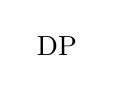
\begin{tikzpicture}[baseline=(root.base)]

        \Tree 	[.\node(root){DP};
                    D
                    [.PossP
                        [.Poss min ]
                        [.NP \edge [roof]; {bil} ]
                    ]
                ]

    \end{tikzpicture}\columnbreak
    \ex
    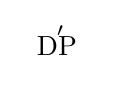
\begin{tikzpicture}[baseline=(root.base)]

        \Tree 	[.\node(root){DP};
                    D
                    [.PossP
                        [.DP \edge [roof]; {min} ]
                        [.Poss$'$
                            Poss
                            [.NP \edge [roof]; {bil} ]
                        ]
                    ]
                ]

    \end{tikzpicture}
    \z\end{multicols}
\z

He presents a number of arguments in favour of this idea.  Specifically, he
demonstrates that while pronominal arguments in other contexts can be somewhat
complex in \ili{Swedish}, possessor pronouns cannot. Consider, for example, \eqref{ex:16.21}
(based on \citealt{Delsing1998}).\largerpage[-3]

\ea Swedish\label{ex:16.21}
    \ea[]{
		\gll {}[ Hela han ] var täckt       av lera  \\
        {} whole he {} was covered of  mud \\
        \glt    `He was all covered in mud.'}
    \ex[*]{
		\gll [ Hela hans ] kropp var täckt  av lera.\\
    {} whole his {} body was covered of mud\\}
	\z
\z\largerpage[-3]

The structure of the subject in (\ref{ex:16.21}a), I assume, is roughly \eqref{ex:16.22}, with a null
D.  The pronoun is, in this case, a noun modified by the adjectival quantifier
\emph{hel} `whole'.\footnote{The string in (\ref{ex:16.21}b) is grammatical with the
    analysis (i).

\begin{exe}
    \exi{(i)}\ili{Swedish}\\
	\gll Hela   [ hans kropp~] var täckt av lera.\\
        whole {} his  body was covered in mud\\
	\glt
\end{exe}

More evidence that the parse [hela hans] kropp is ruled out is provided by
sentence fragments:

\begin{exe}
    \exi{(ii)}\ili{Swedish}\\
    Vems kropp var täckt av lera?\\
        `Whose body was covered in mud?'
    \llap{*}
		\gll Hela hans\\
            whole his\\
\end{exe}}

\ea\label{ex:16.22}
    {}[\textsubscript{DP} D [\textsubscript{NP} hela [\textsubscript{NP} han ]]]
\z

If the pronominal possessor were a DP, (\ref{ex:16.21}b) would arguably be
predicted to be well-formed. If, on the other hand, the pronominal possessor is
a D-type head, it is predicted that it would not be modifiable by an
adjective.\footnote{\citet[227--230]{Julien2005} provides the following example
    to counter \citegen{Delsing1998} claim that prenominal possessor pronouns
    are heads in \ili{Swedish}:

\begin{exe}
    \exi{(i)}\ili{Swedish}\\
	\gll {}[ vårt alla ]-s ansvar \\
        {} our  all \hphantom{]}-’s  responsibility\\
\end{exe}

In this case the possessor pronoun is embedded as specifier of a quantifier in
a QP, with arguably no relation to the NP \emph{ansvar}.  Interestingly the
pronoun has the genitive\is{genitive case} form, rather than the (perhaps) more expected default
form (which would be nominative\is{nominative case} \emph{vi} in Swedish):
?\emph{vi allas ansvar}.}

The following is a piece of evidence of the same kind, but for
English.\footnote{An anonymous referee points out that (i), although quite
    marginal, is still clearly better than (\ref{ex:16.23}b), as we would expect.

\begin{exe}
    \exi{(i)}[?]{the real you’s answer}
\end{exe}

A related construction, interesting in this context, is discussed by
\textcite{TsoulasWoods2019}.

\begin{exe}
    \exi{(ii)} Norman is both of our friends.
\end{exe}

This looks like a clear counterexample to the claim made in the text that the
English genitive\is{genitive case} pronoun is a head taking the possessee NP as
complement. I will put this issue aside in this paper, though.}

\ea\label{ex:16.23}
    \ea[]{I want to hear an answer from the real you.}
    \ex[*]{I want to hear the real your answer.}
	\z
\z

In \ili{English}, too, a pronoun can function as a noun in restricted circumstances.
The structure of \emph{the real you} is, I assume, roughly \eqref{ex:16.24}:

\ea\label{ex:16.24}
    {}[\textsubscript{DP} the [\textsubscript{NP} real [\textsubscript{NP} you ]]]
\z

If the prenominal possessive pronoun were a DP, this would (arguably) predict
that (\ref{ex:16.23}b) would be good, on a par with (\ref{ex:16.23}a).

Since the pronoun in \eqref{ex:16.21} and \eqref{ex:16.23}
exceptionally functions as a noun, there may be other reasons why the
counterpart possessive construction is not good; it could be that the
genitive\is{genitive case} case cannot \enquote{trickle down} as far as to the
head of NP. A more convincing piece of evidence that the possessor pronoun in
English and \ili{Swedish} is not a DP is provided by the observation that it cannot
be an APC.

\ea Swedish\\\label{ex:16.25}
    \gll \llap{*}{}[ våra barn ] åsikter\\
        {} our  children {} opinions\\
    \glt Intended: `we childrens opinions'
\z

\ea[*]{our children opinions}\label{ex:16.26}
\z

\subsection{Coordination of possessor pronouns}\label{sec:16.3.2}

The \ili{English} \isi{coordination} facts mentioned in the introduction provide another
argument that possessor pronouns are not DPs, in \ili{English}. Pronouns that are
subjects or objects can be coordinated, as in \eqref{ex:16.27}, but possessor pronouns
generally cannot, as seen in (\ref{ex:16.28}--\ref{ex:16.29}) \parencite[601--602]{QuirkEtAl1972}:

\ea\label{ex:16.27}
    {}[ You and I ] are friends. They didn’t see [ us or them ].
\z

\ea\label{ex:16.28}
    \judgewidth{??}
    \begin{multicols}{2}
    \ea[??]{my and your (friends)}
    \ex[??]{your and my}
    \ex[??]{my and his}
    \ex[?]{his and my}
    \ex[??]{your and his}
    \ex[?]{his and your}
    \ex[??]{my and her}
    \ex[??]{her and my}
    \ex[??]{your and her}
    \ex[??]{her and your}
    \ex[]{his and her}
    \ex[??]{her and his}
	\z\end{multicols}
\z

\ea\label{ex:16.29}
    \begin{multicols}{2}
    \ea[??]{our and your}
    \ex[??]{your and our}
    \ex[??]{our and their}
    \ex[??]{their and our}
    \ex[??]{your and their}
    \ex[??]{their and your}
	\z\end{multicols}
\z

This is not the full paradigm, as I have not included \isi{coordination} of a
singular and a plural pronoun, nor any \isi{coordination} with \emph{its}. However,
even including them, the generalization is that all coordinations of two
possessor pronouns are degraded, although less with those that have \emph{his}
as the first conjunct (particularly \emph{his and her}). Assigning \enquote{??}
to the rest of them is an idealisation. Speakers tend to agree that they are
degraded, but to somewhat varying degrees. Putting that case of \emph{his}
aside for the moment, if the pronouns are Poss heads in a structure
(\ref{ex:16.20}a), not DPs in a structure (\ref{ex:16.20}b), and in
particular if they are derived by agreement, as will be proposed in the next
section, that could explain why you cannot coordinate them.\footnote{The
    assumption that possessive pronouns are heads does not, on its own, explain
    why they cannot be coordinated, since there is (at least apparently)
    \isi{coordination} of some functional heads\is{functional items}: \emph{if and when (the situation
    changes)}, \emph{She both can and will contest the
    decision}.}\textsuperscript{,}\footnote{\citet{Cardinaletti1998} discusses \isi{coordination} of pronouns in
        \ili{Italian}, and notes that while postnominal possessor pronouns can be
        coordinated, prenominal ones cannot. Her analysis of the prenominal
        ones is not too dissimilar from the one articulated here for \ili{English}
        and \ili{Swedish}: She argues that they are \isi{clitics}, which is what I will
        argue below holds true of the \ili{English} and \ili{Swedish} possessor pronouns,
        albeit in the context of a theory \citep{Roberts2010} where the
        derivation of pronominal \isi{clitics} is different from that in
        \citet{Cardinaletti1998}. As discussed by \citet{CarSta1999}, it is a
        criterial property of weak and clitic pronouns that they cannot be
        coordinated (cf.\ \citealt{Kayne1975};
        \citealt[228--233]{Holmberg1986}). Thus, if the \ili{English} possessive
        pronouns are weak or clitic pronouns we expect them not to be
        coordinatable. However, it is not the case that the extant theories
    actually explain why weak and clitic pronouns cannot be coordinated.}\largerpage[2]

Perhaps surprisingly, in view of the discussion above, \ili{Swedish} allows
coordination of possessor pronouns. \eqref{ex:16.30} only lists three coordinations, but in
fact any combination of two pronouns is good.\footnote{I am indebted to Tom
    Swallow, who conducted a questionnaire-based experiment comparing
    \isi{coordination} of possessive pronouns in \ili{English}, \ili{Swedish}, and \ili{Danish} as part
of his BA degree programme at Newcastle University in 2015.}

\ea\label{ex:16.30}\ili{Swedish}
	\ea
		\gll mina och dina vänner\\
			mine   and  your friends\\
	\ex
		\gll dina och hennes vänner\\
			yours and her friends\\
	\ex
		\gll våra och deras vänner\\
			ours and your friends\\
	\z
\z

Note the glosses. Differently from \ili{English}, the possessor pronouns in \ili{Swedish}
have only one form where \ili{English} has a weak and a strong (independent) form:
\emph{my} vs. \emph{mine}, \emph{your} vs. \emph{yours}, etc. The claim is that
the \ili{Swedish} coordinated pronouns in \eqref{ex:16.30} are coordinated PossPs
each with a pronominal head and an NP, as shown in \eqref{ex:16.31}, where
the NP is elided/null in the first conjunct. I assume the \isi{coordination} as a
whole is a Conjunction phrase (CoP), as in \citet{Johannessen1998}, but this is
not crucial.

\ea\label{ex:16.31}
    {}[\textsubscript{CoP} [\textsubscript{PossP} mina [\textsubscript{NP} vänner]] [och [\textsubscript{PossP} dina [\textsubscript{NP} vänner]]]]
\z

Alternatively the second NP can be deleted, giving \eqref{ex:16.32}:

\ea\label{ex:16.32}\ili{Swedish}\\
	\gll mina vänner och dina\\
		my friends    and yours\\
\z

Many speakers (although not all) agree that the \ili{English} coordinations in \eqref{ex:16.33}
are better than the ones in \eqref{ex:16.28} and \eqref{ex:16.29}, as we would expect, given that they
can be analysed as \isi{coordination} of two PossPs. The structure of, for example,
\emph{mine and your friends} would be roughly \eqref{ex:16.34}.

\ea\label{ex:16.33}
	\ea mine and your friends
	\ex yours and his friends
	\ex hers and his friends
	\ex ours and their friends
	\ex theirs and your friends
	\z
\z

\ea\label{ex:16.34}
    {}[\textsubscript{CoP} [\textsubscript{PossP} mine [\textsubscript{NP} friends]] [and [\textsubscript{PossP} your [\textsubscript{NP} friends]]]]
\z

Now we can understand why \emph{his} is an exception among the possessor
pronouns; see \eqref{ex:16.28}: \emph{his} is the only possessor pronoun which has an
identical strong and weak form.\footnote{ The pronoun \emph{its} also does not
have a distinct weak and strong form. However, this is because it does not have
a strong form: \emph{I like my food and the cat likes his/*its}. Interestingly,
this is as predicted by \citet{Cardinaletti1998} and \citet{CarSta1999}: Strong
pronouns can only have human reference.} We can therefore assume that the
structure of, for example \emph{his and her friends} is roughly
\eqref{ex:16.35}, a \isi{coordination} of two PossPs.

\ea\label{ex:16.35}
{}[\textsubscript{CoP} [\textsubscript{PossP} his [\textsubscript{NP} friends]] [and [\textsubscript{PossP} her [\textsubscript{NP} friends]]]]
\z

Just as in \ili{Swedish}, an alternative to \emph{his and her friends} is \emph{his
friends and hers}, with the same structure \eqref{ex:16.35}, except that the second NP is
deleted/null instead of the first one.\footnote{ One question that remains
unanswered in the present work is why it is that \isi{coordination} of possessive
pronouns is not ruled out altogether and uniformly, by \ili{English} speakers. It is
possible that coordinations like \emph{my and your friends} can be analysed, at
least by some speakers, as \isi{coordination} of two DPs: [\textsubscript{DP} my
friends] and [\textsubscript{DP} your friends], with exceptional deletion of
the NP in the first conjunct; exceptional because a null NP normally requires
the strong form pronoun \emph{mine}. I leave this matter for future research.}

Coordination of possessive pronouns in \ili{English} is discussed in
\citet{Payne2011}. Payne notes first that \textcite{QuirkEtAl1972} classifies them as
ungrammatical. In a search of the British National Corpus he finds 12 examples
of coordinated possessive pronouns, five of which are \emph{his and her}. He
takes this as evidence that \isi{coordination} of possessive pronouns is not
ungrammatical, and he proceeds to propose a syntactic analysis for them. In the
spring of 2017, I did a search of coordinated possessive pronouns in a number
of \ili{English} corpora together with a group of students as part of an advanced
syntax course at Newcastle University. Our findings were consistent with
Payne’s: a small quantity of examples were found in every corpus, proportional
to the size of the corpus. For example the Corpus of Contemporary American
English (COCA, then 520,000,000 words) contained 15 tokens of \emph{your and
my}, 13 of which were in the relevant context: \emph{your and my} NP. We then
did a comparison with a \ili{Swedish} corpus, using the corpus search engine KORP,
accessing a range of \ili{Swedish} corpora. We picked the corpus
\emph{Tidningstexter} `Newspaper texts' as it was roughly the same size as COCA
(just over 592,000,000 words) and a similar genre, contemporary written
sources. There were 235 tokens of \emph{din och min} `your/yours and my/mine',
166 of which were relevant. This gives a clear indication of how many examples
you expect to find of this construction in a language where it is grammatical:
more than 12 times as many as in \ili{English}. We can only conclude that it is a
marginal construction, at best, in \ili{English}, unlike, for example, \ili{Swedish}. This
is what needs to be explained.

\subsection{Agree in the possessive construction}\label{sec:16.3.3}

\citet{Delsing1998} studiously avoids taking a stand on what the source of the
pronominal Poss head is. Following standard assumptions within phrase structure
theory in general and \citet{Roberts2010} in particular, I will assume that a
head cannot itself be an argument. It can, however, agree with an argument,
which is what happens in the PossP. The argument agreed with may itself be
null, as for example in the case of a null subject\is{null subjects} in agreement with T in
languages with rich subject--verb agreement
\citep[passim]{BibHolRobShee2010}.  This is also the case in the PossP.
I take the structure of the PossP \emph{our home} to be \eqref{ex:16.36},
at the point when Poss is merged with NP.

\ea\label{ex:16.36}
    \begin{tikzpicture}[baseline=(root.base), align=center]

        \Tree 	[.\node(root){PossP};
                    {Poss\\uφ\\\glsunset{EPP}\gls{EPP}}
                    [.NP
                        \Fpl{}
                        [.N home ]
                    ]
                ]

    \end{tikzpicture}
\z

The structure is, again, somewhat simplified. The NP that Poss merges with is
more accurately a Num(ber)P, as mentioned earlier. The possessor argument, in
this case, a bare pronoun, which I take, for now, to be made up of just the
valued \isi{φ-features} [\First,\Pl{}]. I shall refer to it as φP, a maximal category
(though not actually a phrase; see \cref{fn:16.19}). The φP is assigned a role by N; I
refer to it loosely as a possessor role.\footnote{This includes any role that
    can be assigned by a noun, including agent or theme (\emph{their discovery
    of a new planet}, \emph{my release from prison}, etc.).
    \citet{AleHaeSta2007} postulate a head within what is called NP here,
    distinct from N, which introduces a possessor argument. They call this head
    Poss, not to be confused with the head Poss in the present model. Such a
    head could be assumed here, but would potentially increase the number of
parameters more than is needed to account for the observations here, and will
therefore not be assumed.\label{fn:16.18}}

The head of PossP has the features [Poss, uφ] and an \gls{EPP}\is{extended
projection principle} feature. The presence of uφ-features in Poss in \ili{English}
is a new hypothesis, to be tested here. It is less controversial in the case of
Finnish and \ili{Hungarian}, as will be discussed below.

Due to its uφ-features, Poss will probe its complement NP seeking a set of
valued \isi{φ-features}. In the case of \eqref{ex:16.36}, it will find the φ-feature set [\Fpl{}]
and copy its feature values. As a result, and since the φP in \eqref{ex:16.36} has no
lexical content, after valuation the feature values of the pronoun will be a
proper subset of the feature values of Poss.

Following \textcite{Roberts2010,Roberts2010b}, this means that the φP is formally a copy of Poss.
The possessor pronoun and Poss form a chain of two copies, equivalent, in
relevant respects, to a chain derived by \isi{movement}, although in this case the
chain is derived by Agree alone.\footnote{The fact that the lower copy is a
    maximal category while the higher copy is a head is no obstacle. The lower
    copy, the pronoun, is in fact a minimal-maximal category
    \citep[249]{Chomsky1995}. A category α is minimal if it dominates no
    category distinct from α, and maximal if it is not immediately
    dominated by a category non-distinct from α
    \citep[54--56]{Roberts2010}. The pronoun meets both conditions. All that
matters for incorporation in Roberts’s sense is the feature
content.\label{fn:16.19}} \textcite{Roberts2010,Roberts2010b} refers to this as incorporation: The φP is incorporated in the head
Poss. As is generally the case in chains, only one copy is spelled out,
typically the higher copy. So the copy that is \enquote{deleted}, i.e.\  not
spelled out, in this case is the φP. The resulting structure is
\eqref{ex:16.37}. A morphological rule spells out the feature complex
[Poss,D,\Fpl{}] as \emph{our}. Note that there is no Case-feature involved;
incorporation ensures that the resulting chain is visible to the morphological
rules spelling out the pronoun (essentially as predicted by
\citealt[117--119]{Baker1988}).

\ea\label{ex:16.37}
    {}[\textsubscript{PossP} [Poss, D, \Fpl{}] [\textsubscript{NP} [\sout{\Fpl}]
        home]]] $\rightarrow$ \emph{our home}
\z

Consider \ili{Finnish}. The counterpart of \emph{our home} is \eqref{ex:16.38}:

\ea\label{ex:16.38} \ili{Finnish}\\
    \gll (meidän) koti-mme\\
        \hphantom{(}our home-\Fpl{}\\
\z

The underlying structure is, again, \eqref{ex:16.36}. Consider first the option with no
spelled out pronoun. As in \ili{English}, [uφ] probes and finds the valued \isi{φ-features}
of the possessor pronoun. The values are copied. Since the pronoun is now a
copy of the Poss head, it will be deleted, i.e.\ not spelled out in PF. The
features are spelled out on Poss. The head Poss itself is spelled out as a
suffix on the noun. While it may be attractive to think that the suffixation is
a result of \isi{head movement} of the noun to Poss (in particular as \ili{Finnish} has
\isi{head movement} in other constructions; see~\citealt{HolmbergEtAl1993}), the fact that
adjectives and quantifiers precede the noun militates against such an analysis.

\ea Finnish\\\label{ex:16.39}
	(meidän) uusi kotimme\\
	'our new home'\\
\z

I therefore assume some form of affix lowering from Poss to N to derive the
suffixed noun form.

As \eqref{ex:16.38} and \eqref{ex:16.39} show, the pronoun can optionally be spelled out, with genitive
Case. I assume the genitive\is{genitive case} Case is assigned by N to its specifier, the
possessor (more on this below). I assume the optionality of spell-out is
because the pronoun has a [uCase] feature optionally. If it does not, it will
be deleted after Agree, as a copy of Poss. If it does, it will be spelled out,
as the Case-feature will rule out \isi{copy deletion} (assuming that the Poss does
not have a genitive\is{genitive case} feature).  Also, if it is not deleted, the \gls{EPP}\is{extended projection principle} will trigger
movement of it from NP to the spec of PossP, shown by the fact that it precedes
the adjective, an adjunct to NP, in \eqref{ex:16.39}. The structure of \eqref{ex:16.39} will be \eqref{ex:16.40},
if the Case option is taken.

\ea\label{ex:16.40}
    {}[\textsubscript{PossP} [\Fpl{}, \Gen{}] [\textsubscript{Poss$'$}
        [Poss, \Fpl{}] [ [\textsubscript{AP} uusi]
        [\textsubscript{NP} [\sout{\Fpl{}, \Gen{}}] koti ]]]]
\z

If the possessor is a lexical DP, there is no agreement, no copying of
φ-features between Poss and the possessor, neither in \ili{English} nor in \ili{Finnish}.
In \ili{English} this results in the spell-out of the \isi{φ-features} of Poss as
\emph{-s}, the default spell-out. In \ili{Finnish} it is spelled out as absence of a
possessor suffix and presence of genitive\is{genitive case} morphological case\is{case!morphological case}
on the possessor noun and its specifiers. Why is there no copying of
φ-features? An initially plausible hypothesis is that this is because a lexical
DP does not have the φ-feature that Poss wants, namely person, assuming that
the third person of a lexical DP is = no person (cf.\
\citealt{HarRit2002,Nevins2007} for discussion). Consideration of the
possessor-\gls{APC}\is{adnominal pronoun construction} indicates that this is
not the reason, though. The possessor-\gls{APC}\is{adnominal pronoun
construction}, being headed by a D encoding \Fpl{} or \Spl{}, has person, yet
does not trigger agreement.  If there was agreement between Poss and a lexical
possessor, with or without \gls{APC}\is{adnominal pronoun construction}, the
result would look like (\ref{ex:16.41}a,b), following \gls{EPP}-driven
movement of the possessor argument to the spec of PossP. The structure of
(\ref{ex:16.41}b) would be (\ref{ex:16.41}c).\footnote{The well-formed
    expression (i) contains the string \emph{we children our home}. It does
    not, however, form a constituent. Instead, \emph{we children} is a hanging
    topic. Example (ii) shows the effect when the string is analysed as a
    constituent.

\begin{exe}
    \exi{(i)}[]{We/us children, our home is important to us.}
    \exi{(ii)}[*]{They didn’t like we/us children our home.}
\end{exe}}

\ea\label{ex:16.41}
    \ea[*]{the girl her car}
    \ex[*]{we children our home}
    \ex[]{[\textsubscript{PossP} [we children]
            [\textsubscript{Poss$'$} our [\textsubscript{NP} \tuple{we children}
                [\textsubscript{N$'$} home]]]]}
	\z
\z

This construction is in fact found in late 16th and 17th century \ili{English}, the
so called \enquote{his-genitive}.

\ea\label{ex:16.42}\textcite[ex. 5]{Allen2002}\\
	and then is there good vse of Pallas her Glasse\\
	`and then there is good use made of Pallas' mirror'
\z

As noted by \citet{Allen2002}, a construction like it is found in some other
Germanic languages as well: \ili{Norwegian}, \ili{Afrikaans}, \ili{Dutch} and \ili{German}. Note,
however, that in those languages the pronoun which, by hypothesis, spells out
Poss is a reflexive pronoun which does not agree with the possessor. Even
though the pronoun in 16th-17th century \ili{English} did agree with the possessor,
as shown by \citet{Allen2002}, it seems that this is a marked
phenomenon.\footnote{ The following sentence, found on the web (thanks to Marit
    Julien for data and discussion) shows what a genitive\is{genitive case}
    \gls{APC}\is{adnominal pronoun construction} looks like in \ili{Norwegian}, when
    employing the \enquote{his-genitive}.

\begin{exe}%(i)
    \exi{(i)} \ili{Norwegian}\\
	\gll Tror    nok  både hennes eget og   oss barn     sine             liv    ville               vært bedre.\\
		think \Ptcl{} both  her  own  and us children their.\Refl{} lives would.have been better\\
	\glt    `I do think both her own life and the lives of us children would have been better.'
\z

The pronoun realizing Poss in the \ili{Norwegian} his-genitive is a reflexive which
agrees with the possessee NP but not with the possessor, at least not directly;
if the possessor is a pronoun it will agree with  the possessee NP, hence
indirectly with the reflexive.}

In \ili{Finnish}, the absence of agreement between Poss and the possessor shows in
the absence of an agreement suffix on the possessee noun.

\ea\label{ex:16.43}Finnish\\
    \ea
		\gll lapsien             koti(*-nsa)\\
		        children.\Gen{} home-\Third{}\\
	\ex
		\gll meidän    lapsien            koti(*-mme)\\
			we.\Gen{} children.\Gen{} home-\Fpl{}\\
	\z
\z

We also need to account for another difference between \ili{English} and \ili{Finnish}
visible when comparing (\ref{ex:16.43}b) and \eqref{ex:16.44} (cf.
\ref{ex:16.2}a).

\ea[*]{our children home}\label{ex:16.44}
\z

The \gls{APC}\is{adnominal pronoun construction} can have a genitive\is{genitive case} head in \ili{Finnish} but not in \ili{English}. As
discussed in \Cref{sec:16.2}, \ili{Swedish} patterns like \ili{English} in this
respect, while \ili{Hungarian} patterns like \ili{Finnish} in the case when the possessor
has dative case.

I propose that what blocks agreement between Poss and the lexical possessor in
English and \ili{Finnish} is genitive\is{genitive case} Case. Just like oblique Case
assigned to a subject blocks agreement between T and the subject, as seen very
clearly in \ili{Icelandic} \citep{Thrainsson2007}, but also in \ili{Finnish}
\parencites{LaitinenVilkuna1993}[209--210]{Holmberg2010b}, genitive\is{genitive
case} Case assigned to the possessor blocks agreement between Poss and the
possessor. I propose, furthermore, that the formal mechanism blocking the
agreement is a Case head K at the head of the possessor argument, intervening
between Poss and D.

\ea\label{ex:16.45}
    \begin{tikzpicture}[baseline=(root.base), align=center]

        \Tree 	[.\node(root){PossP};
                    \node (poss) {Poss\\uφ\\\gls{EPP}};
                    [.NP
                        [.KP
                            {K\\\Gen}
                            [.DP
                                \node (dp) {DP\\\Fpl{}};
                                [.N children ]
                            ]
                        ]
                        [.NP [.N home ] ]
                    ]
                ]

        \draw (poss.south) |- (dp.west)
            node [midway, fill=white] {\ding{55}};

    \end{tikzpicture}
\z

I assume KP is assigned genitive\is{genitive case} by N, along with the possessor theta role.
Poss probes, but K blocks access to the \isi{φ-features} of D, with the result that
[uφ] of Poss is spelled out as \emph{-s}.\footnote{ A slightly different formal
account is that the probing [uφ] finds the Case-feature [\Gen{}] of K, and
copies this feature. Under this analysis, the \emph{-s} would be a
morphological realization of genitive, as in traditional grammatical
description.} The \gls{EPP}\is{extended projection principle} steps into action and triggers \isi{movement} of KP to merge
again with PossP, deriving \emph{we children’s home} or \emph{us children’s
home}, depending on which form of the pronoun is the default (which varies
across dialects and idiolects).

One crucial difference between \ili{English} and \ili{Finnish} is that \ili{Finnish} has
morphological case on nouns and specifiers of nouns. As in \ili{English}, N assigns
genitive Case to KP. In \ili{Finnish} this Case trickles down to D, with its person
and number feature, and to N. As in \ili{English}, Poss probes, but access to the
φ-features of D is blocked by K. The result is that the [uφ]-features of Poss
are ignored at both interfaces, LF and PF (there is no \enquote{crash}; see
\citealt{Preminger2014}). The \gls{EPP}\is{extended projection principle}
triggers \isi{movement} and remerge of the KP with PossP. The valued Case-features of
the noun and the possessor features are spelled out as genitive.

If this is on the right track, then the pronominal form \emph{meidän} `our' in
Finnish has two derivations: (a) The genitive\is{genitive case} Case can be assigned directly by
the possessee N to a bare pronoun. In that case Poss can agree with the
genitive pronoun, or (b) it can be assigned by N to a KP containing a
possessive pronoun along with a lexical NP, and trickle down from KP to the
pronoun. In that case there is no agreement between Poss and the head of the
possessor, seen most clearly in the case of the \gls{APC}\is{adnominal pronoun construction} possessor. In \ili{English}
there is one derivation only: the possessive pronoun is the spellout of
agreement between Poss and the possessor.\footnote{The difference between
pronouns and lexical DPs in the way they agree with the Poss head in the
possessive construction does not have an obvious analogue in subject
agreement\is{agreement!subject agreement}
with T in the languages discussed here, but is found in some languages,
including \ili{Irish} and \ili{Welsh}, where there is subject--verb
agreement\is{agreement!subject agreement} only with
pronominal subjects. If we follow \citet[128--139]{Roberts2010} and analyse
object \isi{clitics} in \ili{Romance} languages as the spell-out of agreement between v and
the object, then there is a possible analogue to possessor-Poss agreement in
the \ili{Romance} varieties which do not allow \isi{clitic doubling}, including French and
varieties of \ili{Spanish} and \ili{Italian}. In those languages v agrees with the object,
agreement realised as a pronominal clitic, only if the object is a pronoun. In
other varieties there is, or can be, agreement also when the object is a
lexical DP; they have so-called clitic doubling.}

\subsection{A note on Hungarian}\label{sec:16.3.4}

In \Cref{sec:16.2} we saw that \ili{Hungarian} shows essentially the same
pattern as \ili{Finnish}, particularly in the case where the possessor has
dative\is{dative case} case. Like Finnish, \ili{Hungarian} has possessor
agreement, spelled out as a suffix on the possessee noun, when the possessor is
a pronoun, not when it is a lexical DP.

\ea\label{ex:16.46}\ili{Hungarian}
   	\ea
		\gll nektek    a    vélemény-e-tek\\
		        you.\Dat{} the opinion-\Poss-\Spl{}\\
	    \glt `your opinion'
	\ex
		\gll a    gyerekeknek    a    vélemény-e\\
			the children.\Dat{} the opinion-\Poss{}\\
		\glt `the children's opinion'
	\z
\z

As in \ili{Finnish}, the possessor can be an \gls{APC}\is{adnominal pronoun
construction}, but only when it has dative\is{dative case} case.  On the
assumption that nominative\is{nominative case} case on the possessor, which is
the other alternative in the \ili{Hungarian} possessive construction, means no
case,  the \ili{Hungarian} \gls{APC}\is{adnominal pronoun construction}
conforms with the generalization \eqref{ex:16.18}, repeated here:

\ea\label{ex:16.47}
    An \gls{APC}\is{adnominal pronoun construction} can be a possessor argument if and only if the possessor is assigned
    morphological case\is{case!morphological case}.
\z

And just as in \ili{Finnish}, when the possessor is an \gls{APC}\is{adnominal
pronoun construction}, there is no possessor agreement. The
\gls{APC}\is{adnominal pronoun construction} behaves like a lexical DP in spite
of being headed by a pronoun.

\ea\label{ex:16.48}\ili{Hungarian}\\
    \gll   \llap{?}csak \textbf{nektek} \textbf{gyerekeknek} a véleménye(*-tek) befolyásolja a döntésünket.\\
            only you.\Dat{} children.\Dat{} the opinion.\Poss{}-\Spl{} influences the decision.\Acc{}\\
    \glt    `It's only you children's opinion that influences our decision.'
\z

As in \ili{Finnish}, as well as (although less conspicuously) in \ili{English} and \ili{Swedish},
this is due to conditions on Agree between Poss and the possessor argument. In
English an effect of this is that possessor pronouns cannot be coordinated. In
Finnish and \ili{Hungarian} an effect is absence of a possessor agreement suffix. For
reasons of space I will not discuss the details of the \ili{Hungarian} possessive
construction here.

\section{Conclusions}\label{sec:16.4}

Probably the most controversial claim in this paper is that the possessor
pronoun in \ili{English} (\emph{my}, \emph{your}, \emph{our}, etc.) is the spell-out
of a possessive D-head derived by Agree with an abstract possessor DP within
NP, within the theory of agreement articulated in
\textcite{Roberts2010,Roberts2010b}.  \citet{Delsing1998} argued that the
possessive pronoun in \ili{Swedish} is a head, not an XP, but left open what the
relation is between this head and the possessor argument within NP. The
relation is Agree, valuation of unvalued \isi{φ-features}. As in certain other
cases of Agree, only pronominal arguments can be goals.

Possessor agreement is familiar from languages which exhibit an affix on the
possessee noun agreeing with the possessor. Two such languages are discussed
here, \ili{Finnish} and \ili{Hungarian}. Essentially the same phenomenon can be seen in
these languages: only pronominal possessors trigger agreement, that is
uφ-feature valuation, on a probing head.

The theory can explain why \isi{coordination} of possessive pronouns (\emph{my and
your}, \emph{her and his}, etc.) are typically judged as degraded in \ili{English}.
Possessive pronouns in \ili{English} are realizations of a functional head\is{functional items}.
Coordination of functional heads\is{functional items} is a highly restricted phenomenon (but not
unheard of; for instance auxiliaries in \ili{English} can be coordinated). However,
in this case the \isi{coordination} of pronouns would have to be the result of Agree
between Poss, containing a set of uφ-features, and a possessor CoP in NP; very
likely not an operation provided for by UG.

In \ili{Swedish} \isi{coordination} of possessive pronouns (\emph{min och din} `my and
your', etc.) is perfectly grammatical. However, this is because the \ili{Swedish}
possessive pronouns can all take a null NP complement, unlike the \ili{English}
\enquote{weak form} pronouns (there is no distinction between \emph{my} and
\emph{mine} in Swedish). The coordinated pronouns can therefore always be
analysed as \isi{coordination} of PossPs, in \ili{Swedish}. This also explains why
\emph{his} is the \ili{English} pronoun which is most amenable to \isi{coordination} as the
first conjunct.  This is because \emph{his} is the one pronoun whose strong
form is the same as the weak form.

Another fact that the theory can explain is why the adnominal pronoun
construction (\gls{APC}\is{adnominal pronoun construction}), for example
\emph{we children}, cannot have the head assigned genitive\is{genitive case}
case, in \ili{English} or \ili{Swedish}: \emph{*our children home}. Only Poss, the head of
a possessive construction, can have that form. In \ili{Finnish} the APC can have
genitive\is{genitive case} case and be possessor. Likewise in \ili{Hungarian} the
\gls{APC}\is{adnominal pronoun construction} can be possessor provided it has
dative case. The \gls{APC}\is{adnominal pronoun construction} does not trigger
possessor agreement, though, in \ili{Finnish} or \ili{Hungarian}. That is to say, neither
in \ili{English} and \ili{Swedish} on the one hand or \ili{Finnish} and \ili{Hungarian} on the other
hand can Poss agree with the head of the APC; it is treated as a lexical,
personless DP. By hypothesis, this is because it is assigned
genitive\is{genitive case} Case by N, taking the form of a head K, intervening
and blocking Agree between Poss and the D of the Possessor. In \ili{Finnish} and
Hungarian, but not in \ili{English} or \ili{Swedish}, the Case assigned by N can trickle
down to, and be spelled out on, the D and the N of the possessor, also when it
is an \gls{APC}\is{adnominal pronoun construction}, allowing it to function as
a nominal argument with a Case-marked head.

Throughout the paper I have assumed that a bare possessive pronoun in \ili{English}
or \ili{Swedish} consists of \isi{φ-features} only. A more articulated analysis would
include a null N or null root merged with the φ-feature set, as in
\citet{Panagiotidis2002}, \citet{Elbourne2008}, \citet{HolmbergPhimsawat2017}.
This would complicate the condition on incorporation somewhat; we would need to
postulate that the \isi{copy deletion} operation does not see the null root. This
would seem to be more of a technical than a substantive problem, though.

\printchapterglossary{}

\section*{Acknowledgements}

The inspiration for this paper comes from a conversation with Ian Roberts and
Michelle Sheehan during a walk up the hill to the restaurant from Henk and
Elizabeth's Villa Salmi in Arezzo. We were comparing judgments of various
combinations of coordinated possessive pronouns in \ili{English}, puzzled by finding
that most of them didn’t sound so good. Thanks also to my other colleagues on
the ReCoS team in the relevant period, Theresa Biberauer, Jenneke van der Wal,
Sam Wolfe, and especially Georg Höhn, the world's number one expert on APCs.
Many thanks to the students on the module \enquote{Syntactic puzzles and how to
    solve them} at Newcastle University in the spring of 2016 and 2017 for
    their contribution to the issue of coordinated pronouns, and to all
    colleagues who have supplied judgements. Special thanks to Balázs Surányi
    for his insightful observations regarding \ili{Hungarian} possessives, which were
    crucial for how the story evolved. Finally, thanks to two anonymous
    referees, whose comments and critique led to considerable improvement of
    the paper.

{\sloppy
\printbibliography[heading=subbibliography,notkeyword=this]
}

\end{document}
